%Etude des solutions de réalisation technique possible
%Choix technologique retenus
%Justification de ces choix avec avantages et inconvénients

\subsection{Taxonomie}%Martin
L'ajout d'une taxonomie aux documents permet d'affiner considérablement la recherche.
La taxonomie est un ensemble de mot fermé et fixe donnant une définition très précise, si ce n'est trop rigide aux documents.
En somme, il s'agit d'un système de tagging de documents. 

Si ce genre de structure de données permet généralement l'utilisation d'un apprentissage supervisé, ou un modèle d'apprentissage profond apprendrait par l'exemple à associer a un document une ou plusieurs taxonomie, \textit{via} un \textit{embedding} comme doc2vec\cite{doc2vec} par exemple, ce genre de système était immédiatement exclu dû a la très grande quantité de taxonomies existante pour un document, mais aussi et surtout parce que nous ne possédions pas de corpus de données annotés.
Le temps étant une ressource précieuse dans ce projet, nous ne pouvions nous attarder sur la synthèse d'un tel corpus et nous avions du nous intéresser a des méthodes de classification non supervisé et des techniques du domaine du \textit{Natural Language Processing}

Le but de ce module étant d'associer à des documents des mots provenant d'une taxonomie, nous avons commencé par étudier la possibilité d'utiliser un word2vec\cite{word2vec} ou un doc2vec de facon non supervisé.
L'idée générale de word2vec et de doc2vec est d'associer a un mot ou a un paragraphe/document un vecteur de taille fixe, généralement avec une centaine de dimension. Cette association, ou \textit{embedding}, est apprise du contexte du mot ou du document.
En somme, des mots partageant le même contexte, e.g.\ parent/père auront des vecteurs de mots qui seront proche selon une métrique choisie.
En général, nous utilisons la mesure de la similarité cosinus, donnée par la formule suivante:

\begin{equation}
	\text{similarité} = \frac{\vec{A} \dot \vec{B}}{\norm{\vec{A}}\norm{\vec{B}}}
\end{equation}
où $A, B  \in \mathbb{R}^n$. Cette mesure renvoie un réel compris entre $[-1, 1]$

Cette mesure nous permet d'avoir une mesure de la similarité de deux mots ou groupes de mots.
Idéalement deux mots ayant un sens similaire auront une mesure proche de 1 entre leur deux vecteurs respectifs.
A l'inverse des mots ayant des sens opposé auront une mesure se rapprochant de -1. 

Nous voulions utiliser cette propriété pour obtenir des taxonomies a partir du texte du document.
En analysant chaque mot du document initial et en le passant par un word2vec, nous pouvions obtenir un \textit{embedding} du mot et le comparer avec la banque taxonomique, et donner au documents les mots de la taxonomie ayant une distance faible. 

\begin{figure}[h!]
  \centering
  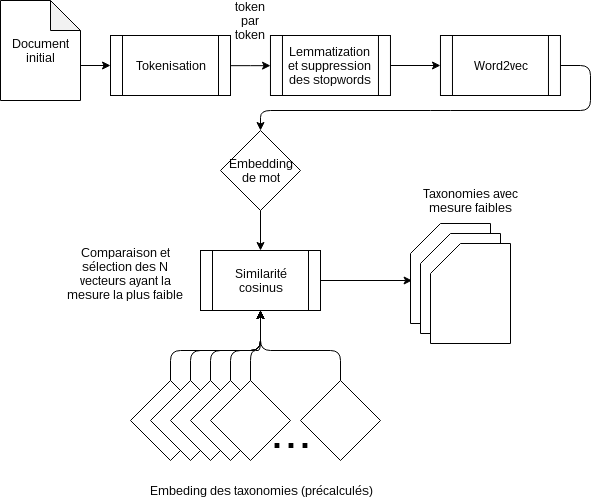
\includegraphics[width=0.8\textwidth]{taxoSchemaFoncInit.png}
	\caption[]{Schéma fonctionnel du module d'assignement taxonomique initial}
  \label{taxoInit}
\end{figure}


Nous avons rencontrés deux problème majeurs avec cette technique.
D'abord, le temps d'execution de cette méthode pour un seul document sur le texte en entier dépassait largement les limites de l'acceptable.
En effet, un document administratif est presque par nécessité très verbeux, et donc long. La majorité du texte ne nous est cependant pas utile pour notre but; 
il ne sert qu'à donner du contexte pour le lecteur et ne donne pas forcément d'information concernant le sujet du document en lui même. 

Deuxièmement, nous n'avons pas pu obtenir les résultats escomptés.
Le principal obstacle venant du fait que les mots de la taxonomie peuvent être en fait des phrases, ou tout du moins de multiples mots dont les sens ne sont pas forcément corrélés.
On trouve par exemple "amménagement foncier", mais aussi "fromage au lait cru" ou bien encore "médecine physique et de réadaptation".
La technique que nous utilisions pour obtenir les \textit{embeddings}, word2vec, ne fonctionne pas sur des \textit{groupes de mots} ou \textit{n-grammes}, mais sur des mots seuls.
doc2vec, qui lui peut fonctionner sur des n-grammes, voires des paragraphes ou documents entier a besoin d'être entrainé sur des documents qui lui apporteront le contexte nécessaire pour former des \textit{embeddings} correct.
Cependant, la taxonomie ne donne aucun contexte.
Il s'agit seulement d'une liste de mot et de phrase ordonnée seulement sous la forme d'un arbre.
Il ne s'agit pas d'un document ordinaire, et nous pouvions pas utiliser les techniques courantes dans ce cas. 

Pour essayer de contrer ce problème, la décision initale fut de transformer chaque mot de la phrase en sa racine par le procédé de la lemmatization a l'aide de la librairie spacy\cite{spacy} et d'enlever les \textit{stopwords} de la phrase.
Les \textit{stopwords} sont des mots apparant très fréquement dans les phrases, comme les déterminants.
Ainsi la phrase "médecine physique et de réadaptation" se trouve transformée en "médecine physique réadaptation".
On utilise ensuite un word2vec sur chaque mot pour obtenir plusieurs vecteurs. Pour obtenir un seul vecteur que nous comparerons avec les mots du documents, nous effectuons un simple moyennage.
Cependant, cette solution n'as pas fonctionné et les taxonomies que nous trouvions a l'aide de ce système ne correspondait simplement pas au document. 

La solution finale adaptée fut celle de simplement extraire les titres d'arrétées administratifs, qui sont les documents a classer, et a les prétraiter par lemmatization et élimination des stopwords avant d'effectuer une simple recherche dans la taxonomie.
Si un mot de la taxonomie se trouve dans le titre de l'article administratif, alors celui ci est ajouté au document.
Cette solution est non seulement bien plus simple et permet de vérifier la qualité des résultats plus aisément qu'à l'aide d'un \textit{embedding}, et elle est de plus bien plus rapide, permettant l'analyse d'un document entier en quelques secondes à peine contre plusieurs minutes a l'aide d'un word2vec.

\begin{figure}[h!]
  \centering
  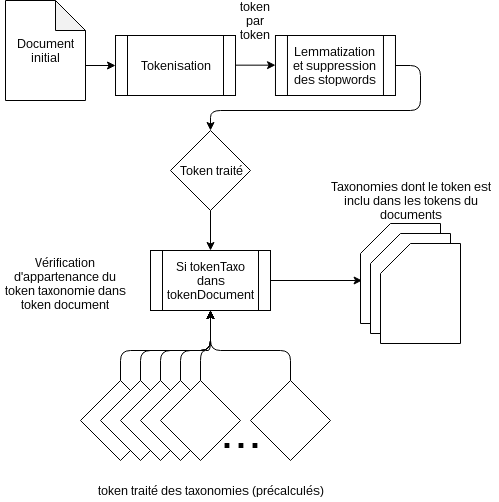
\includegraphics[width=0.8\textwidth]{diagFinalTaxo.png}
	\caption[]{Schéma fonctionnel du module d'assignement taxonomique final}
  \label{taxoFinal}
\end{figure}

On notera que le système final n'utilise pas d'apprentissage.
On peut y voir ici une piste d'amélioration: avec un corpus de données annotés, il devient trivial de construire un module taxonomique plus précis et performant, car prenant en compte le contexte, crucial dans le NLP.
En effet, notre système ne peut distinguer "outre mer" de "mer". Si ces deux exemples contiennent le mot "mer", il est évident que leur sens sémantique est différent.
Ce sens ne peut être compris que par le contexte; fonctionnalité qui manque a ce module. 




\subsection{Recherche de informations d'importance} %Baptiste
Chaque document contient des informations d'importance qui doivent être extraites pour que le document en question soit correctement classé par la suite.
Les informations d'importance, déterminées avec le commanditaire, sont les suivante :
\begin {itemize}
\item La référence du RAA
\item La date de publication
\item Les dates
\item Les références des arrêtés
\item Les références des décrets
\item Les références des articles
\item Les références des lois
\item Les noms des parties prenantes
\item Les lieux
\end {itemize}

 

\subsection{Moteur de recherche} %Stab
\subsubsection{Elasticsearch/Kibana}
Le moteur de recherche est la résultante visuelle de toutes les tâches techniques précédentes effectuées (reconnaissance des charactères, recherche de mots d’importance et la taxonomie). Après une étude de l’art, nous avions relevé le moteur de recherche Elasticsearch. 
Elasticsearch est moteur de recherche open source basé sous le logiciel Apache Lucene. A l’aide d’un fichier JSON (JavaScript Object Notation) qui nous permet de représenter de l’information structurée, il indexe des documents orientés textes via des requêtes HTTP. Cette approche nous permet de ne pas avoir à nous préoccuper des problématiques complexes d’indexations par score des documents. Plusieurs sociétés, telles que Uber, Stack Overflow ou Udemy se basent sur ce serveur pour la recherche de produits/documents sur leurs sites. 

\begin{figure}[h!]
  \centering
  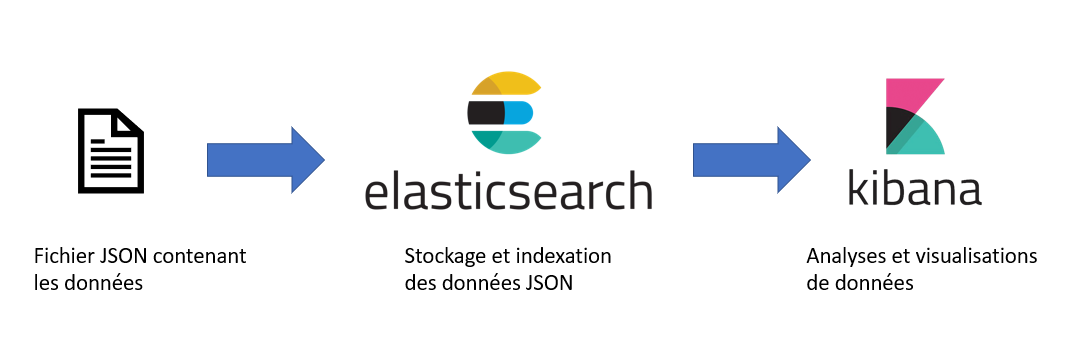
\includegraphics[width=0.8\textwidth]{ArchitectureElasticsearchKibana.PNG}
	\caption[]{Architecture Elasticsearch Kibana}
  \label{}
\end{figure}


Elasticsearch à lui tout seul ne suffit pas pour visualiser ses données depuis un fichier JSON. Comme dit précédemment, c’est à l’aide des requêtes HTTP que l’on peut effectuer une recherche. Par-dessus, nous avons Kibana qui est un greffon de visualisation de données pour Elasticsearch. Il fournit plusieurs fonctions de visualisations et les utilisateurs peuvent créer des diagrammes en bar, en ligne, des nuages de points, des camemberts et des cartes de grands volumes de données avec leurs données JSON.

\begin{figure}[h!]
  \centering
  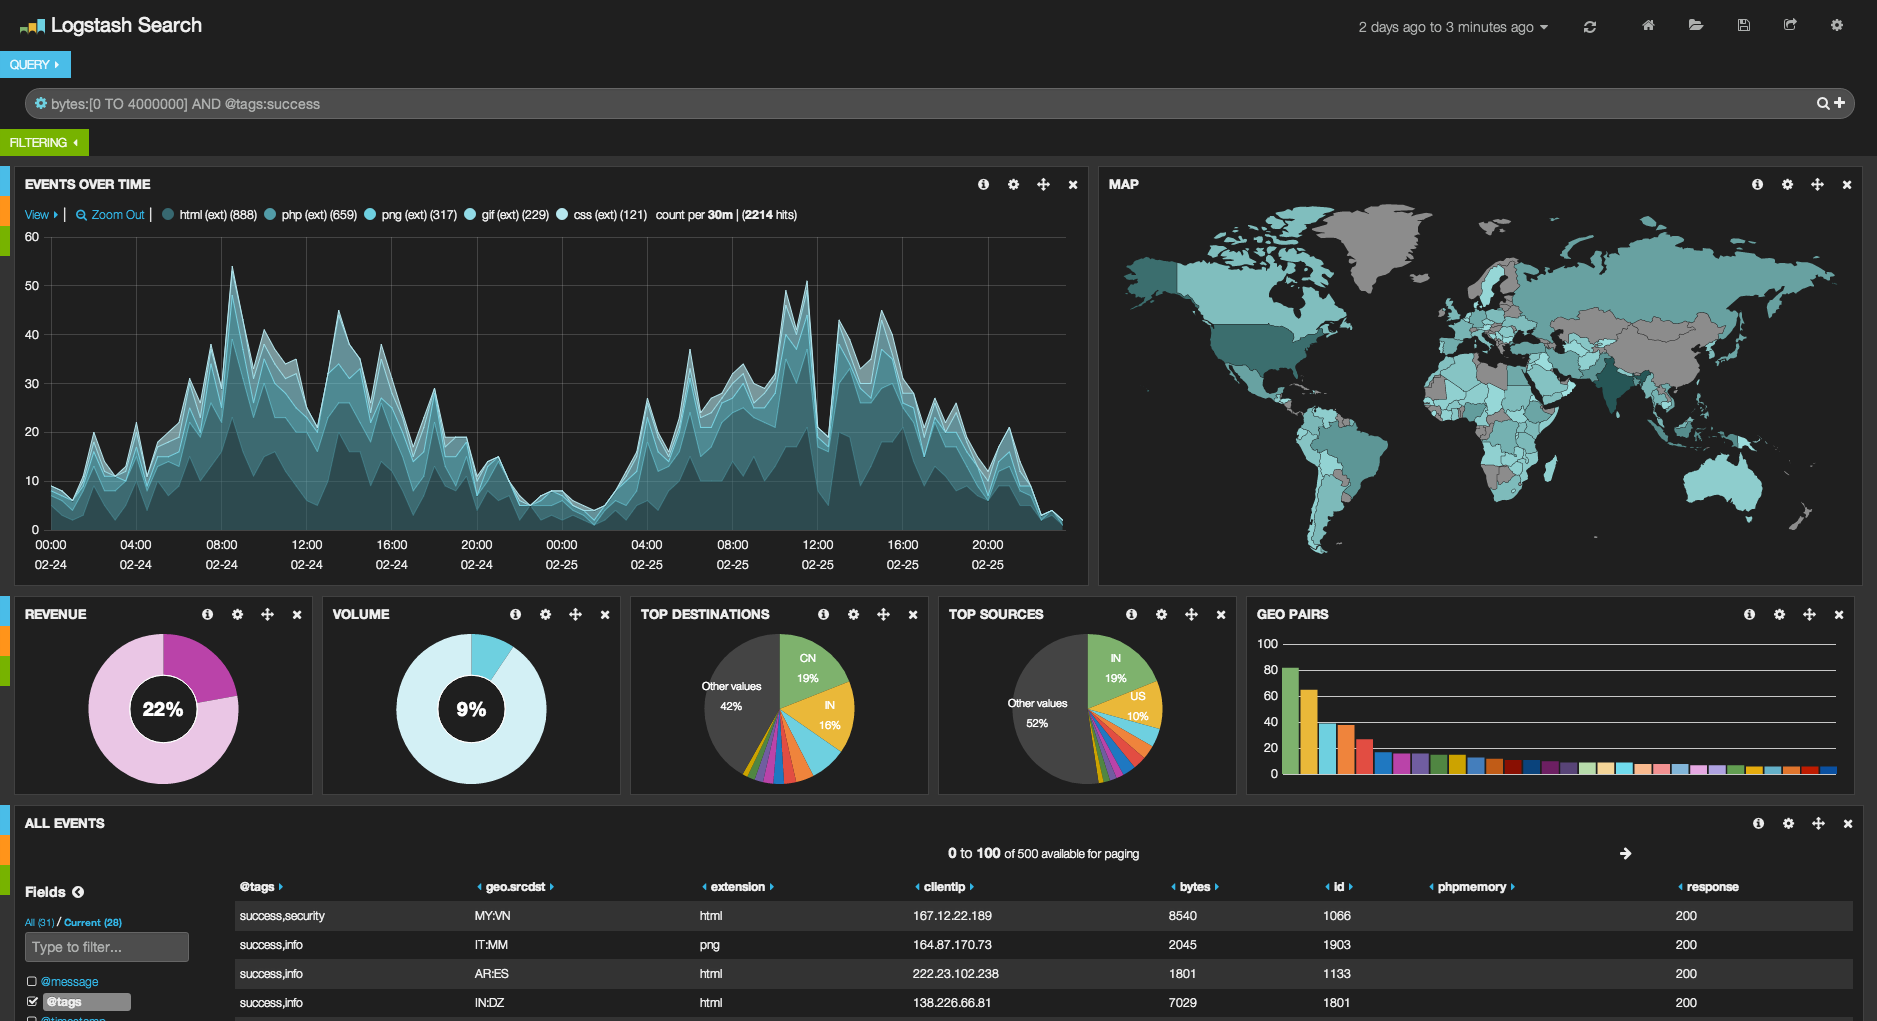
\includegraphics[width=0.8\textwidth]{visualisationKibana.png}
	\caption[]{Exemple de visualisation des données JSON sur Kibana}
  \label{}
\end{figure}


Avec le couple Elasticseach/Kibana, nous avons un moteur de recherche combinée avec une visualisation intéressante. Cela nous évite d’avoir à développer une page web. 
Cependant, cette approche est très orientée analyse de données. Il ne faut pas que l’on oublie que le PoC (\textit{Proof Of Concept}) doit être \textit{user-friendly} pour la préfecture. Premièrement, l’utilisateur doit spécifier son champ de recherche en écrivant fields.champ afin d’effectuer une recherche. Sachant que l’utilisation du moteur de recherche sera effectuée par plusieurs personnes de la préfecture, il serait préférable qu’il soit simple d’utilisation. De plus, comme inconvénient nous avons aussi les fonctionnalités de Kibana qui sont orientés analyse de données.

\begin{itemize}
    \item Avantages 
        \begin{itemize}
            \item Indexation avec elasticsearch
            \item Pas besoin de développer une page web : Visualisation des données avec Kibana
        \end{itemize}
    \item Inconvénient 
        \begin{itemize}
        \item Orienté analyse de données avec Kibana
        \end{itemize}
\end{itemize}

Malgré les multiples avantages, l’inconvénient de la fonctionnalité de Kibana a une importance plus élevée. Même si pour un PoC, cela est présentable mais il est loin d’être ergonomique pour l’utilisateur.
Il faut comprendre que Kibana est une extension d’Elasticsearch. Le seul défaut listé ci-dessus ne concerne que Kibana. Nous avons donc continué nos recherches afin de trouver une extension basée sur Elasticsearch avec une visualisation plus intéressante.

\subsubsection{Reactivesearch/Appbase.io}

Reactivesearch comme son nom l’indique se compose de React et de Elasticsearch. React aussi appelé React.js ou ReactJS est une bibliothèque JavaScript libre développée par Facebook en 2013. Le but principal de cette bibliothèque est de faciliter la création d’application web monopage, via la création de composants dépendant d'un état et générant une page (ou portion) HTML à chaque changement d'état.
Plusieurs sociétés telles que Facebook, Netflix, Yahoo ou WhatsApp l’utilisent. Son avantage est que son implémentation. En une heure nous pouvons avoir un site web. Afin d’arriver à ce résultat, il faut installer ReactivSearch, le connecter avec ElasticSearch, importer nos données JSON puis ajouter les composants UI (User Interface) que nous souhaitons. 
Depuis le site https://appbase.io/ programmé avec ReactivSearch est encore plus intuitif. Ce site permet d’importer des données et d’avoir un template de site monopage avec nos données JSON. De plus, il est possible d’analyser les recherches qui ont été effectué. Appbase se compose d’un 'Daily search volume ' listant l’historique des recherches effectuées sur la page ReactivSearch. 
Lors de l’import des données JSON, nous recevons un mail nous donnant des \textit{credentials} : un ID personnel nous permettant d’accéder au JSON. De cette manière, seules les personnes en possession de cet ID peuvent accéder et développer une page web avec les données importées. 

\begin{figure}[h!]
  \centering
  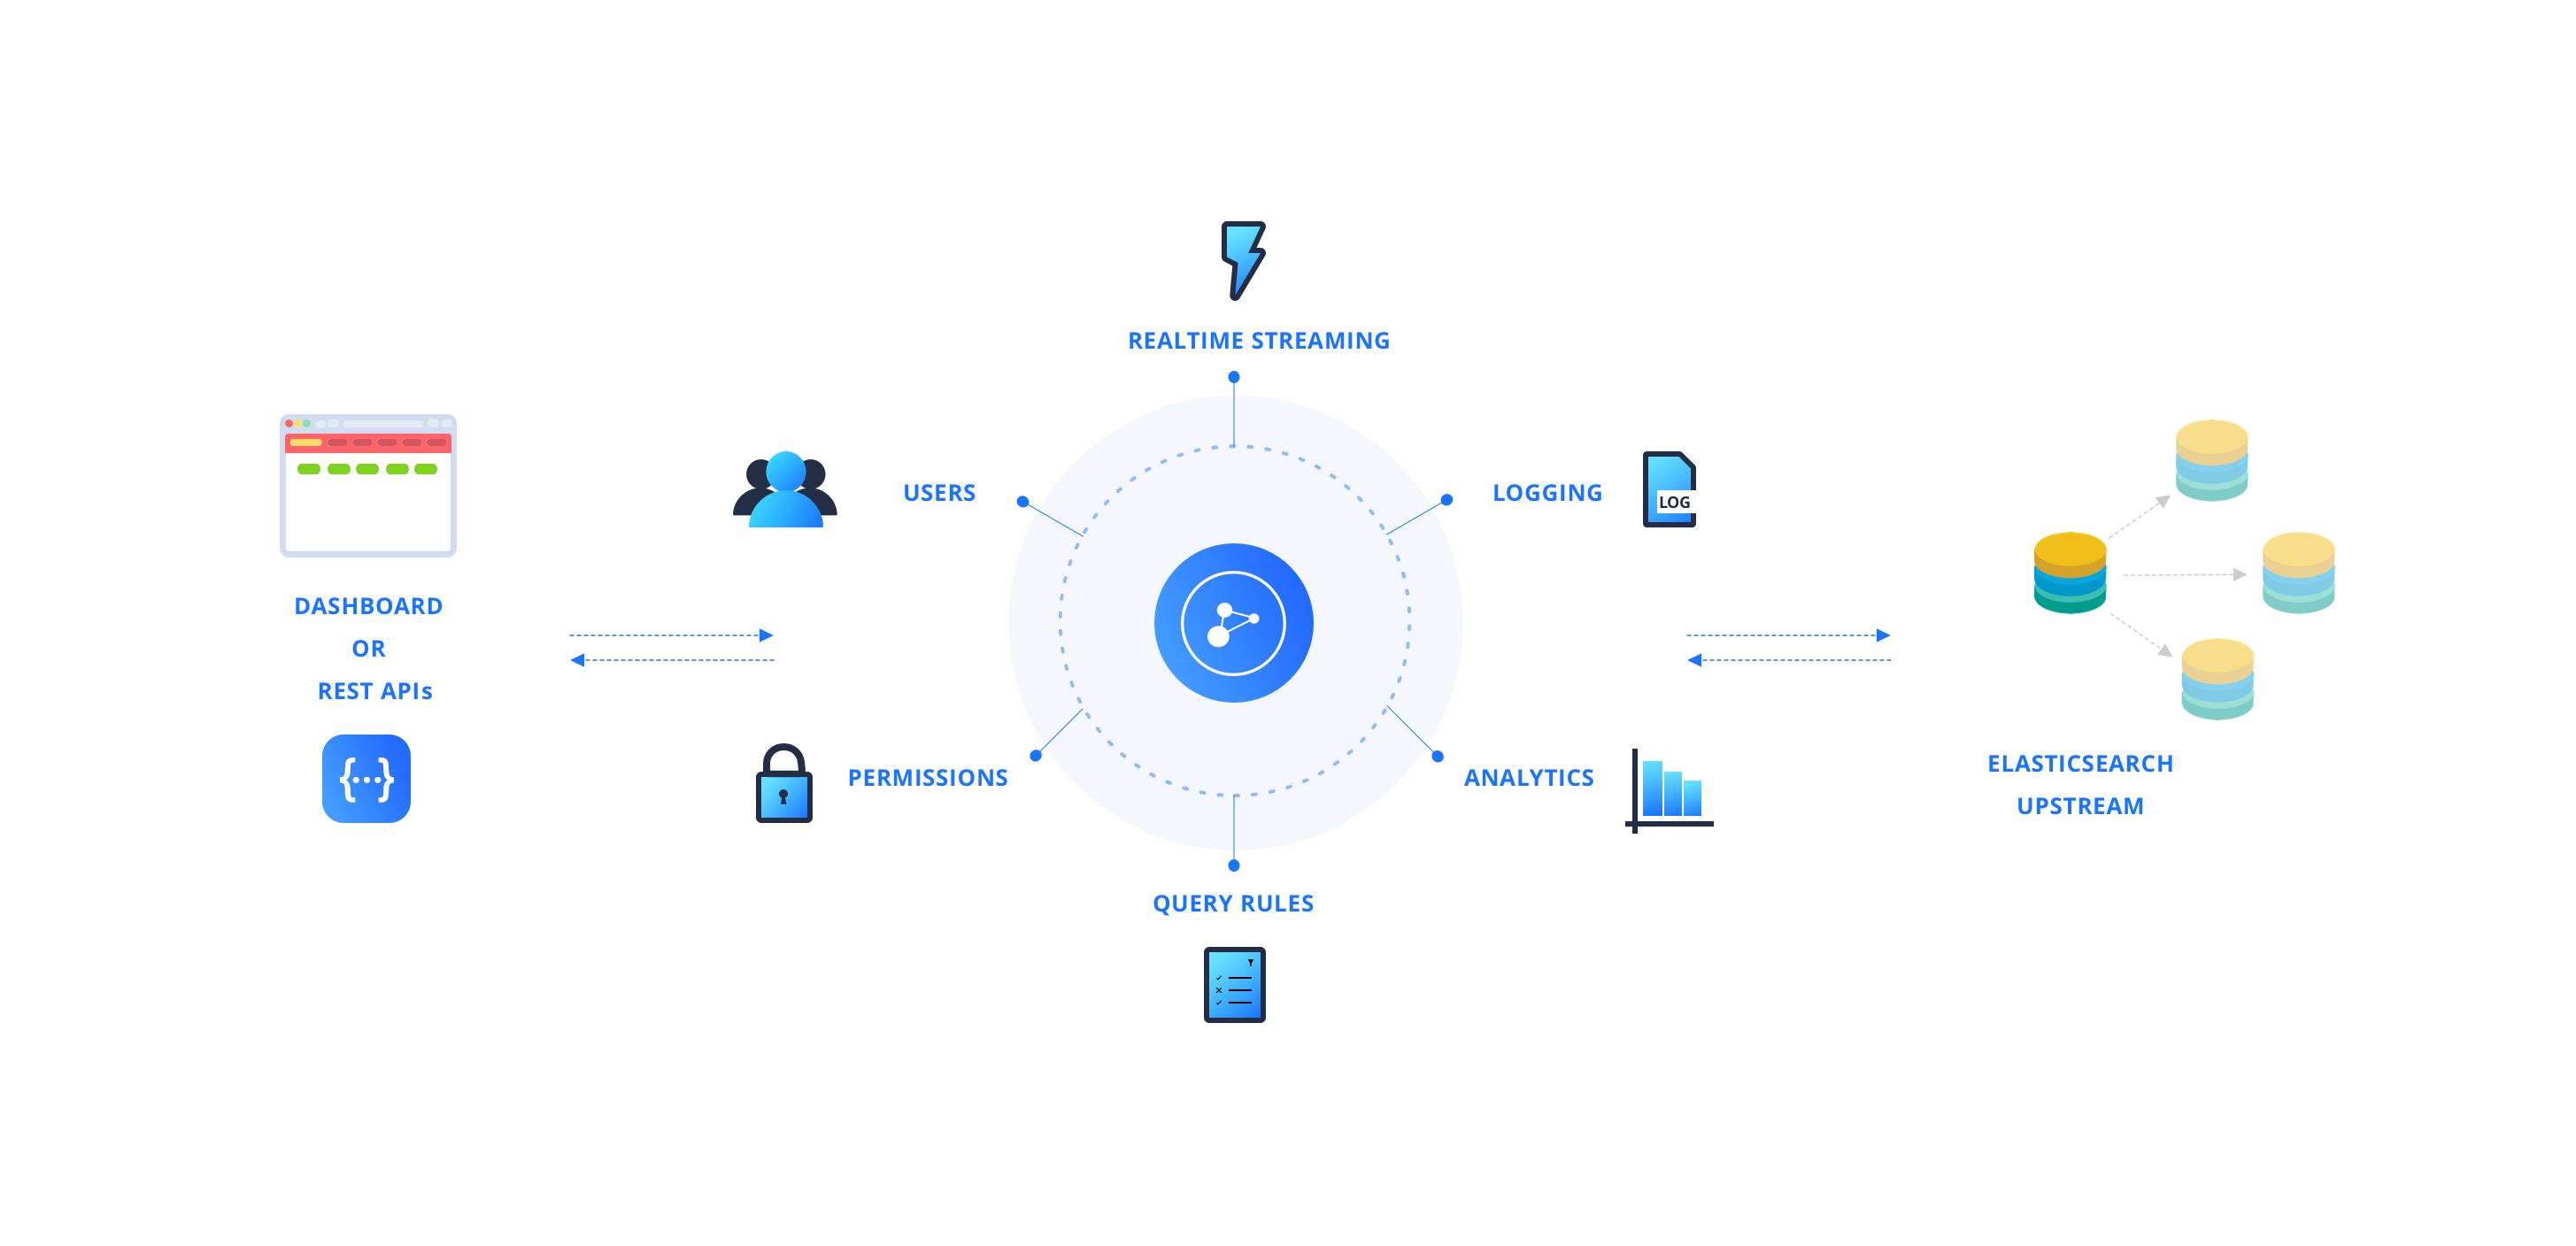
\includegraphics[width=\textwidth]{images/ArchitectureElasticsearchAppbase.png}
	\caption[]{Architecture Appbase.io et Elasticsearch}
  \label{}
\end{figure}

\newpage
\begin{itemize}
    \item Avantages 
        \begin{itemize}
            \item Indexation avec elasticsearch
            \item Simple d’implémentation
            \item Sécurité d’accès aux données avec les credentials
            \item L’analyse des historiques de recherche
            \item Multiplateforme
        \end{itemize}
    \item Inconvénients 
        \begin{itemize}
        \item Monopage
        \item Codes générés à reverse enginneer pour modifier le programme
        \end{itemize}
\end{itemize}

Cette approche d’implémentation répond aux inconvénients de la visualisation avec Kibana. Ainsi son utilisation multiplateforme et facile à prendre en main est le choix que nous avons fait de moteur de recherche.  
